\documentclass[10pt,letterpaper]{article}
\usepackage[letterpaper,top=1.7cm,bottom=1.8cm,left=1.7cm,right=1.7cm]{geometry}
\usepackage{amsmath,amssymb}
\usepackage{booktabs}
\usepackage{graphicx}
\usepackage{times}
\usepackage{url}
\usepackage{cite}
\usepackage{xcolor}
\usepackage{enumitem}
\usepackage{microtype}
\usepackage{hyperref}

\graphicspath{{../visualizations/revision_actual/}}
\setlength{\columnsep}{0.55cm}
\setlength{\parindent}{1em}
\setlength{\parskip}{0pt}
\setlength{\emergencystretch}{2em}
\def\UrlBreaks{\do\/\do-\do_\do.}
\hypersetup{colorlinks=true,linkcolor=black,citecolor=black,urlcolor=blue}

\begin{document}

\section*{Response to Reviewer Comments}
\textbf{Manuscript \#18579}\\
\textbf{Revised title: ``Byzantine-Robust Federated Learning with Adaptive Aggregation and Blockchain: A Reproducible Empirical Evaluation''}

We thank the editor and reviewers for their constructive comments. The manuscript
has been rebuilt around one reproducible experiment rather than combining results
from incompatible configurations. We also removed claims that were not supported
by the final experiment, including the Transparency Paradox, Layer-2 deployment,
production readiness, CIFAR-10 comparisons from legacy scripts, and projected
blockchain costs. The revised manuscript and response are provided in this single
file as requested.

\subsection*{Reviewer A}
\textbf{Comment A1:} ``Attack types are limited to label-flip and random noise;
sophisticated attacks (ALIE [18], backdoor [20]) require future study.'' Rephrase
this as the citations look strange now.

\textbf{Answer:} The limitation is now stated with named authors and methods:
``This study evaluates one combined untargeted attack consisting of cyclic label
flipping and scaled model updates. More sophisticated attacks, including the A
Little Is Enough attack introduced by Baruch et al.~[5] and targeted backdoor
attacks studied by Sun et al.~[6], remain outside the present scope.'' The
references now unambiguously identify the cited attacks.

\textbf{Comment A2:} Figures 1--2 not readable.

\textbf{Answer:} Figures 1 and 2 were regenerated directly from the final
three-seed result file at 300 DPI. Figure 1 reports mean convergence with one
standard-deviation bands. Figure 2 reports final mean accuracy with
$t$-distribution 95\% confidence intervals. Labels, line widths, markers, and
legends were enlarged.

\textbf{Comment A3:} Conclusion (and article) too short I think.

\textbf{Answer:} The manuscript now provides a complete threat model, exact
implementation parameters, formal aggregation equations, a step-by-step
procedure, statistical analysis, measured blockchain evidence, limitations, and
an expanded conclusion.

\textbf{Comment A4:} Expand it to include comparative analysis, contribution
discussion.

\textbf{Answer:} Sections 4 and 5 now compare clean FedAvg, attacked FedAvg,
Krum, TrimmedMean, and ATMA under the same configuration. The discussion
distinguishes accuracy, robustness, adaptation, and auditability. In particular,
we explicitly report that ATMA and static TrimmedMean have statistically
indistinguishable final accuracy in this experiment, while ATMA contributes
automatic trim adaptation and client-level anomaly flags.

\subsection*{Reviewer B}
\textbf{Comment B1:} It is not clear what EXACTLY the authors did and how
(step by step).

\textbf{Answer:} Section 3.7 now lists the executed procedure step by step. The
single experiment uses the actual MNIST dataset, one fixed CNN architecture,
20 clients, full participation, four fixed Byzantine clients, Dirichlet
$\alpha=0.5$ partitioning, 20 rounds, three SGD mini-batches per client per
round, learning rate 0.05, seeds 42/43/44, and the same combined label-flip and
scaled-update attack for all defended and undefended methods. The exact result
artifact is \texttt{results/unified\_mnist\_actual.json}.

\textbf{Comment B2:} There is no point in throwing a lot of terms without being
specific on what you did exactly and how. Not generic information. SPECIFICALLY
in this work.

\textbf{Answer:} Generic and unsupported sections were removed. The revised
methodology defines every transformation, aggregator, statistical calculation,
and blockchain transaction used in this work. The Krum implementation excludes
self-distance and uses $n-f-2$ other neighbors. ATMA is stateful and updates its
trim ratio from the observed robust outlier fraction. Blockchain evidence comes
from an actually deployed Solidity contract on Ganache and includes 420
successful transactions plus deployment, rather than estimated transactions.

\begin{center}
\textbf{REVISED MANUSCRIPT FOLLOWS}
\end{center}

\newpage
\twocolumn[
\begin{center}
{\Large\bfseries Byzantine-Robust Federated Learning with Adaptive Aggregation
and Blockchain: A Reproducible Empirical Evaluation\par}
\vspace{0.5em}
Rachmad Andri Atmoko$^{1,2}$, Sholeh Hadi Pramono$^{1}$,
M. Fauzan Edy Purnomo$^{1}$, Panca Mudjirahardjo$^{1}$,
Mahdin Rohmatillah$^{1}$, and Cries Avian$^{1}$\\
$^{1}$Electrical Engineering Department, Faculty of Engineering,
Universitas Brawijaya, Malang 65145, Indonesia\\
$^{2}$Faculty of Vocational Studies, Universitas Brawijaya,
Malang 65145, Indonesia\\
\textit{Corresponding author: Sholeh Hadi Pramono
(sholehpramono@ub.ac.id)}
\end{center}

\begin{abstract}
Federated learning is vulnerable to Byzantine clients that transmit malicious
model updates. This study presents a reproducible comparison of FedAvg, Krum,
coordinate-wise TrimmedMean, and an adaptive trimmed mean aggregation method
(ATMA), with an Ethereum-compatible audit contract. All methods are evaluated
under one configuration using MNIST, 20 clients, four Byzantine clients,
Dirichlet($\alpha=0.5$) non-IID partitions, full client participation, 20
communication rounds, and seeds 42, 43, and 44. Byzantine clients train on
cyclically flipped labels and scale the transmitted model delta by 5. Clean
FedAvg reaches $82.49\%\pm1.29\%$ final accuracy, whereas attacked FedAvg falls
to $22.36\%\pm2.81\%$. Krum reaches $60.01\%\pm7.37\%$,
TrimmedMean reaches $78.23\%\pm1.51\%$, and ATMA reaches
$78.15\%\pm1.80\%$. ATMA and TrimmedMean are statistically
indistinguishable in final accuracy ($p=0.706$), but ATMA automatically adapts
its per-tail trim ratio from 0.10 toward 0.20 and obtains 96.77\% precision,
100\% recall, and 98.36\% F1 for Byzantine-client flagging over 60 evaluated
rounds. For one ATMA run, a Solidity contract records 400 client-update hashes
and 20 round summaries in 420 successful Ganache transactions. All stored
hashes pass contract read-back verification. These results support robust
aggregation for utility preservation while defining blockchain as an audit
mechanism rather than an accuracy-improving component.
\end{abstract}

\noindent\textbf{Keywords:} federated learning, Byzantine robustness, Krum,
trimmed mean, adaptive aggregation, blockchain auditability
\vspace{1em}
]

\section{Introduction}

Federated learning (FL) trains a shared model from decentralized client data by
aggregating locally computed updates~\cite{mcmahan2017}. Data heterogeneity,
partial trust, and adversarial clients remain central open problems in
FL~\cite{kairouz2021}. A Byzantine client may submit an arbitrary update, so
ordinary weighted averaging can be driven far from the update supported by
honest clients.

Krum selects one update that is geometrically close to other updates and was
introduced as a Byzantine-resilient alternative to linear
aggregation~\cite{blanchard2017}. Coordinate-wise median and trimmed mean
estimators provide another family of robust methods with statistical
guarantees~\cite{yin2018}. These defenses have different behavior under non-IID
data: Krum retains one client update, whereas trimmed estimators combine
coordinate-level information from several clients.

Blockchain has also been proposed as an audit and coordination layer for
FL~\cite{kim2020,lu2020}. It cannot by itself determine whether an update is
malicious, but it can preserve update commitments and aggregation decisions
after an off-chain detector has produced them. This distinction is important:
auditability should not be presented as an improvement in model accuracy.

The contributions of this work are:
\begin{enumerate}[leftmargin=*]
    \item a single controlled comparison of clean FedAvg, attacked FedAvg,
    Krum, TrimmedMean, and ATMA under identical data, model, attack, and
    optimization settings;
    \item a corrected Krum implementation and an explicitly defined adaptive
    trimming rule;
    \item three-seed results with sample standard deviations and
    $t$-distribution confidence intervals;
    \item measured blockchain evidence from a deployed Solidity audit contract,
    including transaction receipts, gas use, and hash read-back verification.
\end{enumerate}

\section{Related Work}

FedAvg computes a sample-weighted average of client updates and is effective
when participants are benign~\cite{mcmahan2017}. It does not provide Byzantine
protection. Blanchard et al.~\cite{blanchard2017} proposed Krum, which scores an
update using its nearest other updates and selects the minimum-score candidate.
Yin et al.~\cite{yin2018} analyzed coordinate-wise robust estimators including
trimmed mean.

Attack strategies extend beyond large outliers. Baruch et
al.~\cite{baruch2019} showed that small, distribution-aware perturbations can
evade several robust rules. Sun et al.~\cite{sun2019} studied targeted backdoor
attacks in FL. The present experiment intentionally uses one transparent,
untargeted attack so that implementation and comparison can be audited; it
does not claim coverage of these stronger attacks.

BlockFL~\cite{kim2020} and blockchain-empowered asynchronous
FL~\cite{lu2020} illustrate how ledgers can exchange, verify, or preserve model
update information. In this work, model training and robust aggregation remain
off-chain. Only SHA-256 commitments, anomaly flags, and round summaries are
stored on-chain.

\section{Methodology}

\subsection{Experimental Protocol}

Table~\ref{tab:configuration} is the single source of truth for all accuracy
comparisons.

\begin{table}[t]
\caption{Unified Experimental Configuration}
\label{tab:configuration}
\centering
\small
\begin{tabular}{ll}
\toprule
Parameter & Value\\
\midrule
Dataset & MNIST, 60,000/10,000\\
Model & CNN, 105,866 parameters\\
Clients & 20\\
Clients per round & 20 (full participation)\\
Byzantine clients & IDs 0--3 (20\%)\\
Data partition & Dirichlet $\alpha=0.5$\\
Communication rounds & 20\\
Local work & 3 mini-batch SGD steps\\
Batch size & 64\\
Learning rate & 0.05\\
Attack scale & 5.0\\
Seeds & 42, 43, 44\\
\bottomrule
\end{tabular}
\end{table}

The model contains two convolutional layers with 16 and 32 channels, two
max-pooling layers, a 64-unit fully connected layer, and a ten-class output
layer. Inputs are normalized with the MNIST mean 0.1307 and standard deviation
0.3081. For each seed, class-specific training indices are divided among 20
clients with a Dirichlet distribution. The same partition and deterministic
mini-batch order are reused across methods for that seed.

\subsection{Threat Model}

Clients 0--3 are Byzantine in every attacked run. During local training, a
Byzantine client replaces each label by
\begin{equation}
y'=(y+1)\bmod 10.
\end{equation}
Let $\Delta_i^t=w_i^t-w^t$ be the local model delta produced from global model
$w^t$. A Byzantine client transmits
\begin{equation}
\widetilde{\Delta}_i^t=5\Delta_i^t,
\end{equation}
thereby amplifying the update learned from poisoned labels. Honest clients
transmit $\Delta_i^t$. The attack is applied in every round. A clean FedAvg run
with identical optimization settings but no Byzantine behavior provides the
upper comparison baseline.

\subsection{FedAvg}

For client sample counts $n_i$, FedAvg computes
\begin{equation}
\Delta_{\mathrm{FA}}^t =
\sum_{i=1}^{N}\frac{n_i}{\sum_j n_j}\Delta_i^t.
\end{equation}

\subsection{Krum}

For $N$ submitted updates and a Byzantine bound $f$, the score of update $i$ is
\begin{equation}
s(i)=\sum_{j\in\mathcal{N}_i}\|\Delta_i^t-\Delta_j^t\|_2^2,
\end{equation}
where $\mathcal{N}_i$ contains the $N-f-2$ nearest \emph{other} updates.
Self-distance is set to infinity before neighbor selection. Krum returns the
single update with minimum score. Here $N=20$ and $f=4$, satisfying
$N\geq2f+3$.

\subsection{Static TrimmedMean}

For coordinate $q$, the 20 scalar values
$\{\Delta_{i,q}^t\}_{i=1}^{20}$ are sorted. Static TrimmedMean removes four
values from each tail and averages the remaining 12:
\begin{equation}
\Delta_{\mathrm{TM},q}^t=
\frac{1}{N-2f}\sum_{i=f+1}^{N-f}\Delta_{(i),q}^t.
\end{equation}

\subsection{Adaptive Trimmed Mean}

ATMA first flattens each update and computes the coordinate-wise median vector
$m^t$. Client distance is
\begin{equation}
d_i^t=\|\Delta_i^t-m^t\|_2.
\end{equation}
Using the median distance $\widetilde d^t$ and median absolute deviation
$\operatorname{MAD}(d^t)$, the robust score is
\begin{equation}
z_i^t =
\frac{d_i^t-\widetilde d^t}
{1.4826\operatorname{MAD}(d^t)+\epsilon}.
\end{equation}
Clients with $z_i^t>3.5$ are flagged. If $\widehat p_t$ is the flagged fraction,
the per-tail trim ratio is updated by
\begin{equation}
r_t=\operatorname{clip}\left[
r_{t-1}+\eta\left(
\operatorname{clip}(\widehat p_t,0.05,0.20)-r_{t-1}
\right),0.05,0.20\right],
\end{equation}
with $r_0=0.10$ and $\eta=0.50$. ATMA then applies coordinate-wise trimmed mean
with $k_t=\operatorname{round}(Nr_t)$ values removed from each tail.

\subsection{Blockchain Audit Contract}

The Solidity contract stores an update-hash mapping indexed by round and
client, the corresponding anomaly flag, and a
round summary containing the aggregate hash and accepted/flagged counts. The
coordinator submits SHA-256 commitments; model tensors are not stored on-chain.
The contract was compiled with Solidity 0.8.19 and deployed to Ganache chain
1337. Blockchain logging was enabled for ATMA with seed 42. Accuracy comparisons
do not use blockchain state and are therefore not attributed to blockchain.

\subsection{Executed Procedure}

For each seed and method, the implementation executes:
\begin{enumerate}[leftmargin=*]
    \item set Python, NumPy, PyTorch, and CUDA seeds;
    \item load and normalize MNIST;
    \item create the seed-specific Dirichlet partition;
    \item initialize the same CNN architecture;
    \item copy the global model to each of the 20 clients;
    \item perform three deterministic mini-batch SGD steps;
    \item poison labels and scale deltas for clients 0--3 in attacked runs;
    \item aggregate all 20 deltas using the selected method;
    \item update and evaluate the global model on all 10,000 test images;
    \item for the audited ATMA run, submit all update hashes and the round
    summary, wait for receipts, and read stored hashes back from the contract;
    \item serialize per-round metrics, metadata, receipts, and summaries to
    \texttt{results/unified\_mnist\_actual.json}.
\end{enumerate}

\subsection{Statistics}

Final accuracy is summarized across three seeds with the sample standard
deviation. The 95\% confidence interval uses Student's $t$ distribution with
two degrees of freedom. Paired, two-sided $t$ tests use seed-matched final
accuracies. Because $n=3$, inferential results are interpreted as supporting
evidence rather than broad population estimates.

\section{Results}

\begin{table}[t]
\caption{Final MNIST Accuracy Across Three Seeds}
\label{tab:actual_results}
\centering
\begin{tabular}{lccc}
\toprule
Method & Mean (\%) & SD & 95\% CI \\
\midrule
FedAvg (clean) & 82.49 & 1.29 & [79.28, 85.69] \\
FedAvg (attack) & 22.36 & 2.81 & [15.39, 29.33] \\
Krum & 60.01 & 7.37 & [41.71, 78.32] \\
TrimmedMean & 78.23 & 1.51 & [74.47, 81.99] \\
ATMA & 78.15 & 1.80 & [73.68, 82.62] \\
\bottomrule
\end{tabular}
\end{table}


The attack reduces FedAvg from 82.49\% to 22.36\%, a mean decrease of 60.12
percentage points. Krum improves attacked accuracy by 37.65 points,
TrimmedMean by 55.87 points, and ATMA by 55.79 points. Seed-paired tests give
$p=0.018$ for Krum versus attacked FedAvg, $p=0.0019$ for TrimmedMean, and
$p=0.0022$ for ATMA. These values should be read cautiously because only three
seeds were evaluated.

\begin{figure}[t]
\centering
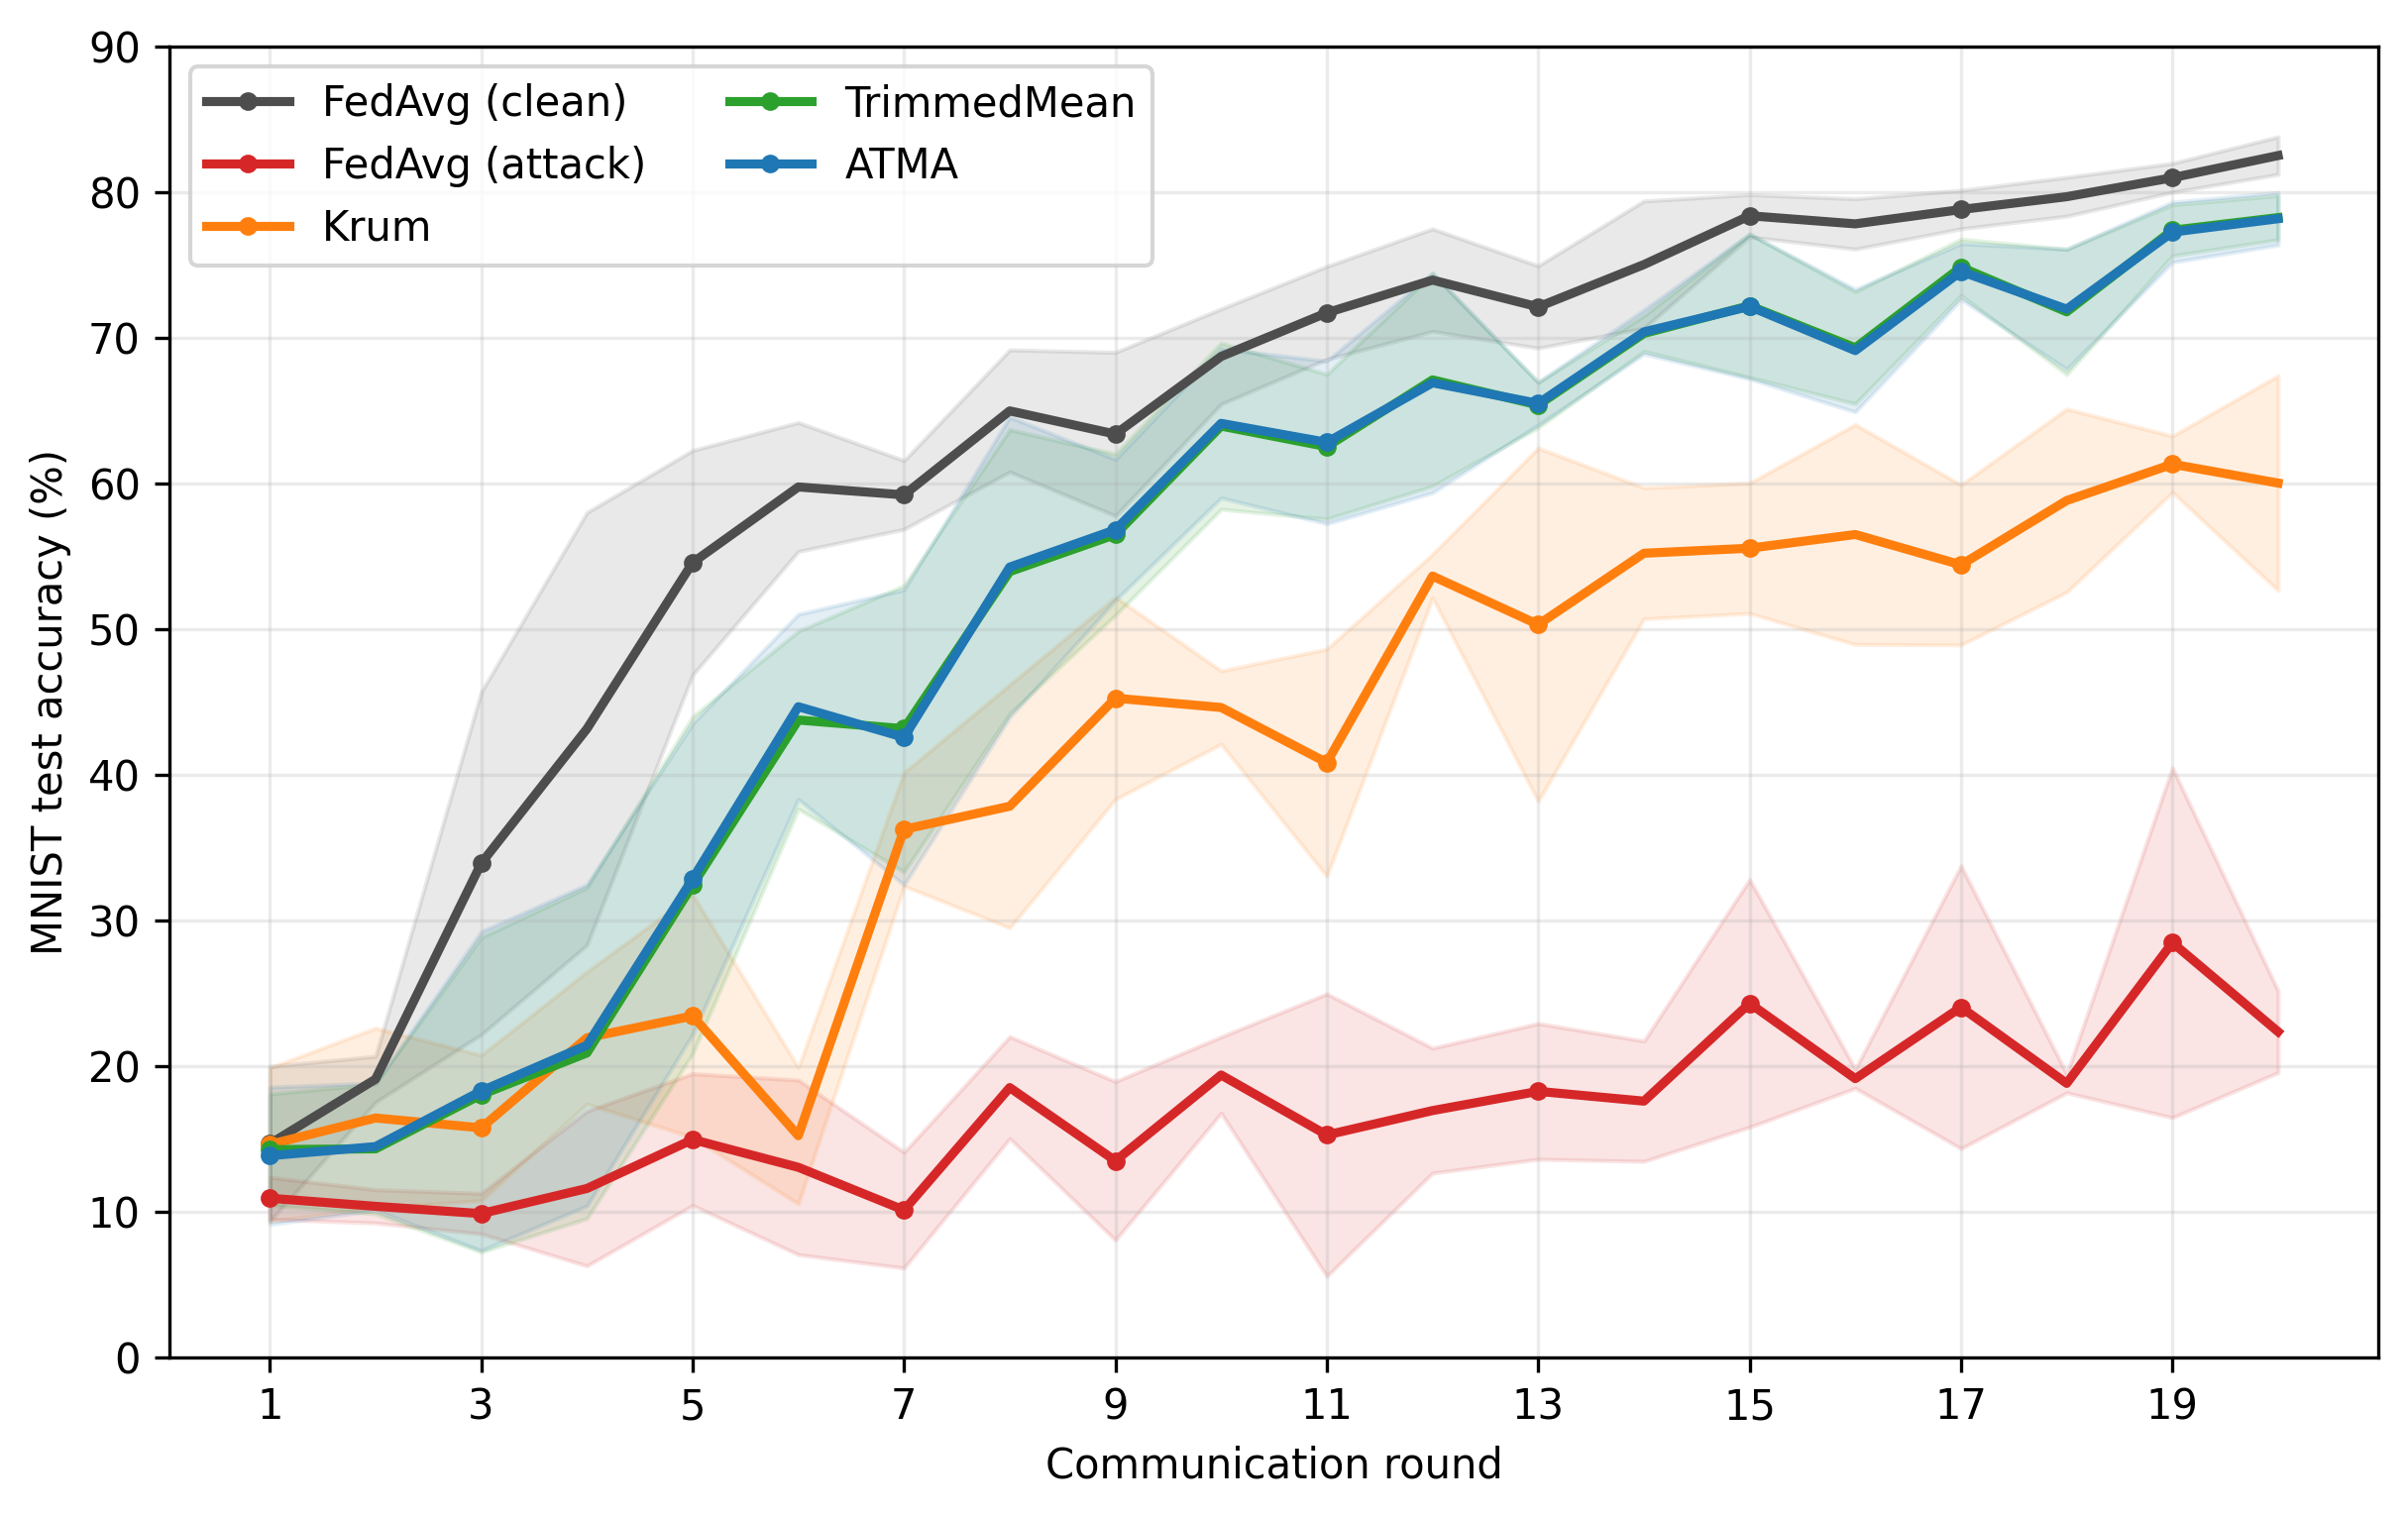
\includegraphics[width=\columnwidth]{figure1_convergence_actual.png}
\caption{Mean test accuracy across seeds 42, 43, and 44. Shaded regions show
one sample standard deviation. Every method uses the configuration in
Table~\ref{tab:configuration}.}
\label{fig:convergence}
\end{figure}

Figure~\ref{fig:convergence} shows that clean FedAvg converges fastest. Attacked
FedAvg remains unstable and low. Krum avoids malicious clients but learns more
slowly because each round retains only one client update. TrimmedMean and ATMA
combine several updates and finish close to the clean baseline.

\begin{figure}[t]
\centering
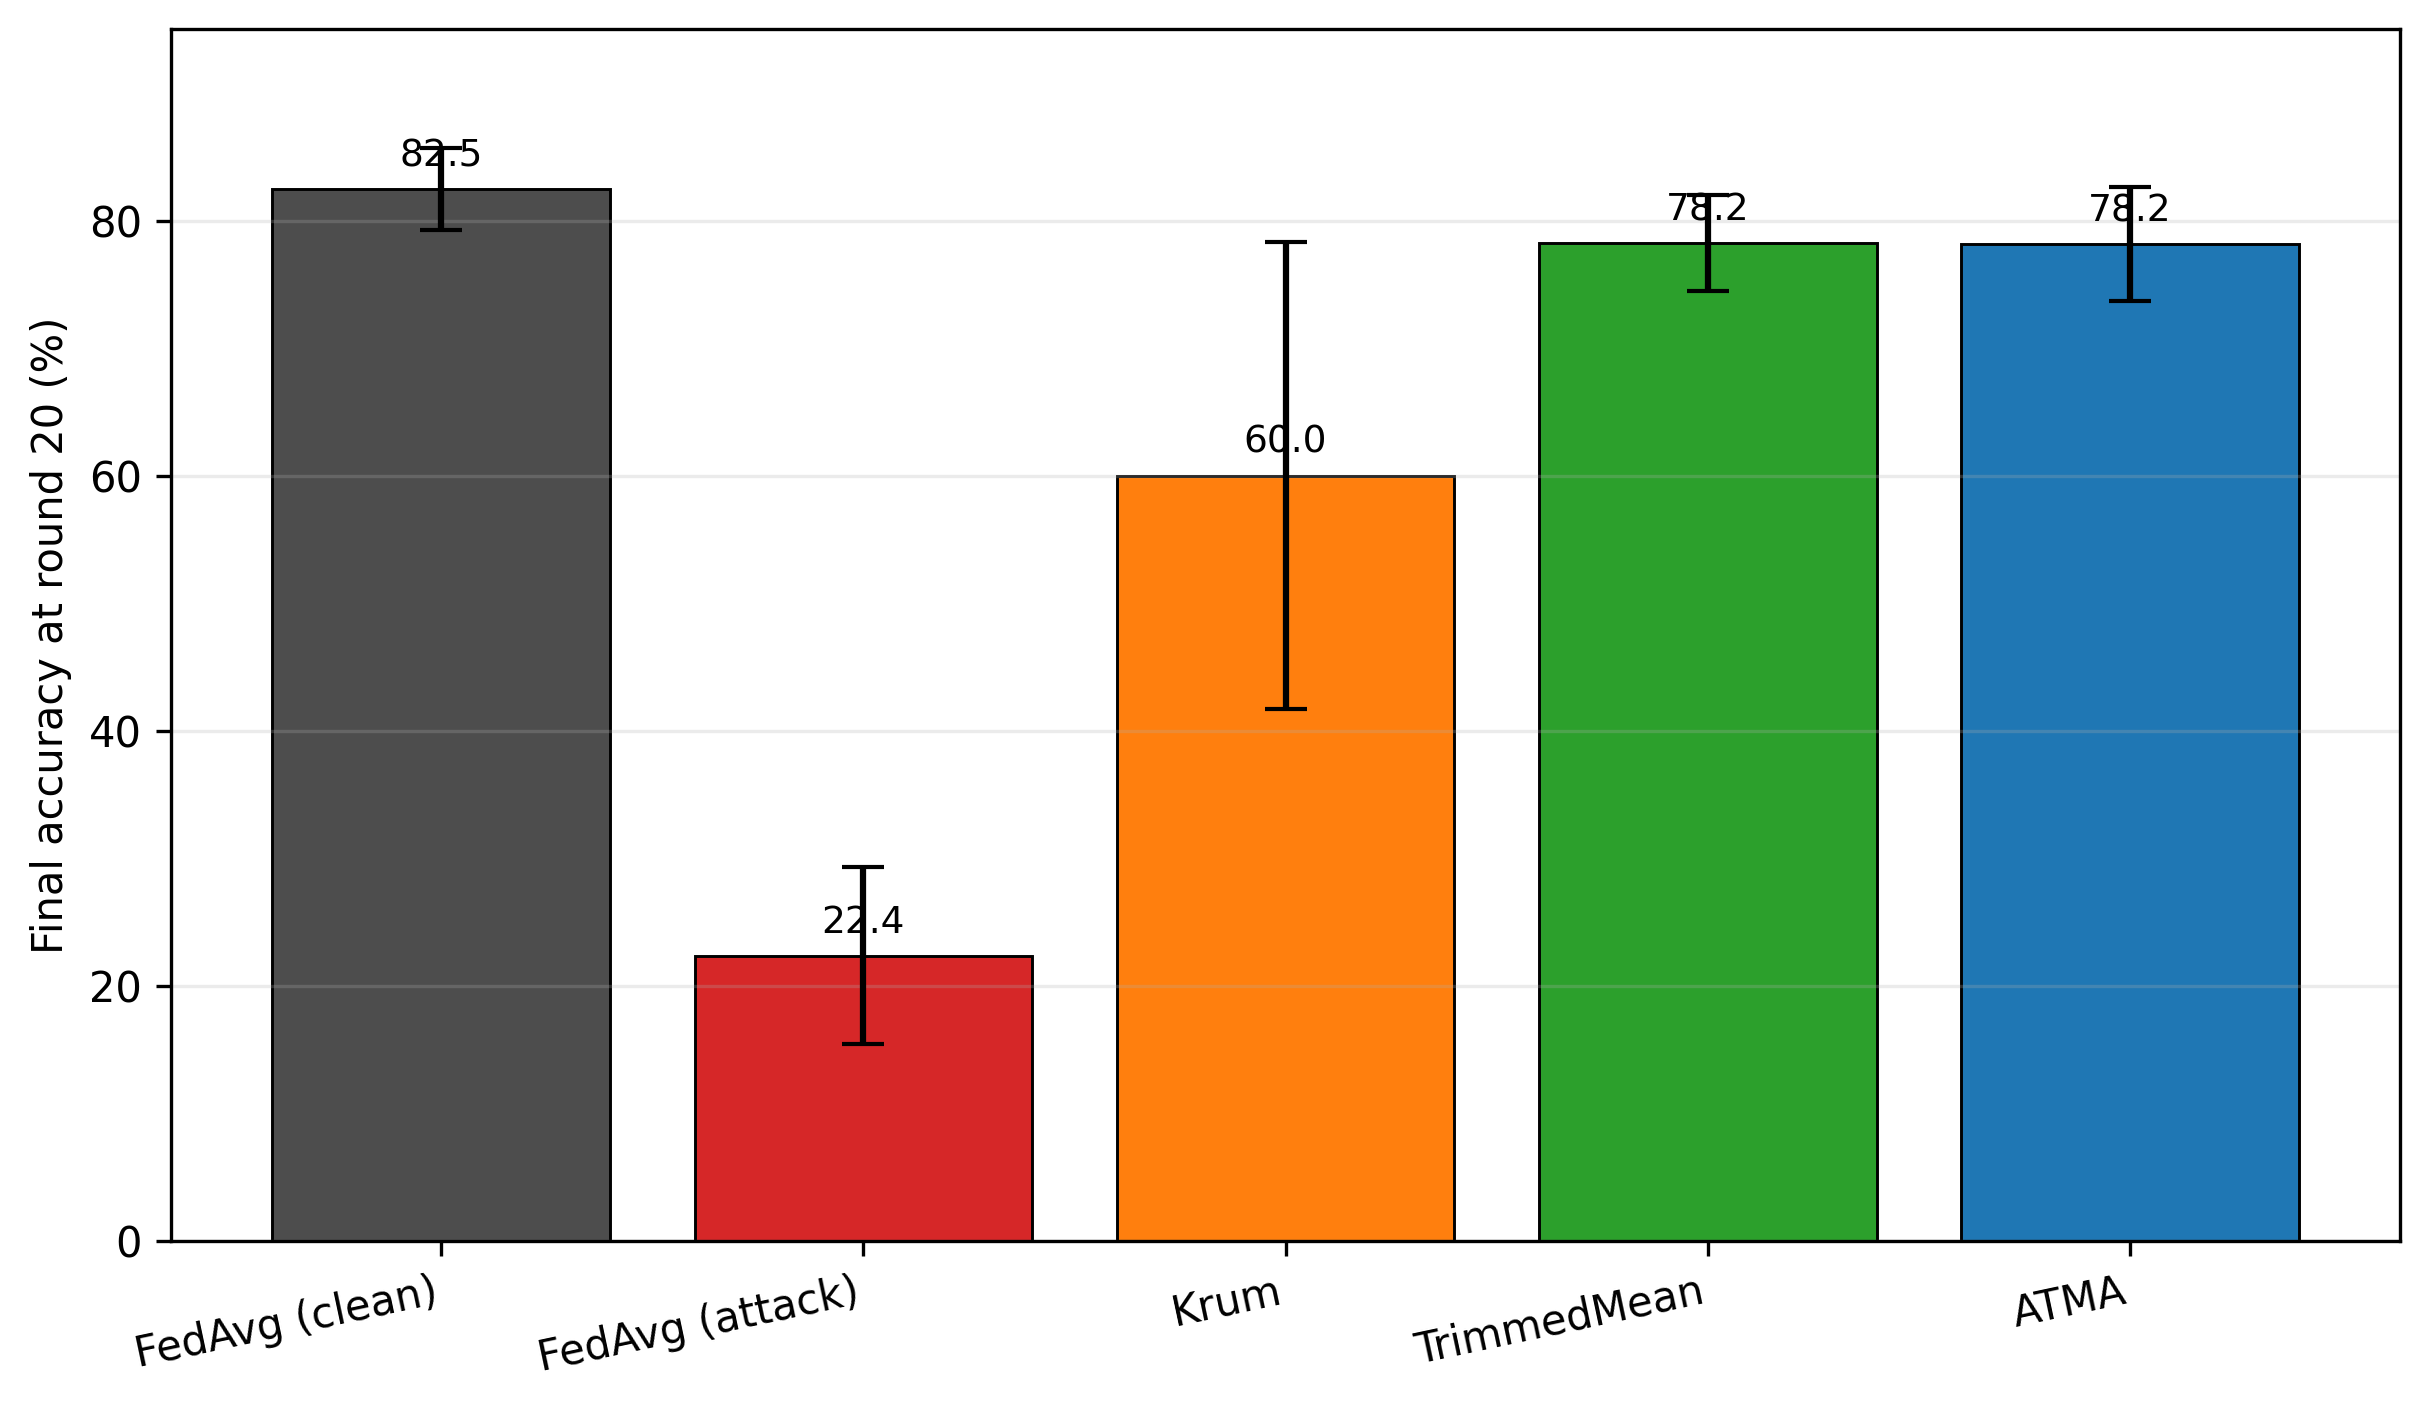
\includegraphics[width=\columnwidth]{figure2_final_accuracy_actual.png}
\caption{Final accuracy at round 20. Error bars are 95\% confidence intervals
computed with Student's $t$ distribution for three seeds.}
\label{fig:final_accuracy}
\end{figure}

ATMA and TrimmedMean differ by only $-0.08$ percentage points on average, with
$p=0.706$. Therefore, this experiment does not establish an ATMA accuracy
advantage. Instead, ATMA removes the need to manually set the final trim count:
its ratio is initialized at 0.10, changes to 0.15 after the first observed
round, and approaches 0.20 in all three runs.

\subsection{Detection and Krum Selection}

Across 60 ATMA rounds, there are 240 Byzantine client-round instances and 960
honest instances. ATMA produces 240 true positives, eight false positives, no
false negatives, and 952 true negatives. Precision is 96.77\%, recall is
100\%, and F1 is 98.36\%. The number of flags per round ranges from four to six.
These metrics concern the explicit attack used here and should not be
generalized to stealthier attacks.

Corrected Krum selects an honest client in all 60 evaluated rounds. Its lower
accuracy therefore does not indicate Byzantine selection; it reflects the
utility cost of reducing a heterogeneous 20-client round to one update.

\subsection{Measured Blockchain Evidence}

\begin{table}[t]
\caption{Measured Ganache Audit Transactions}
\label{tab:blockchain_actual}
\centering
\begin{tabular}{lrr}
\toprule
Operation & Count & Mean Gas \\
\midrule
Contract deployment & 1 & 512,965 \\
Client update record & 400 & 54056 \\
Round finalization & 20 & 113991 \\
\midrule
Total measured gas & -- & 24,415,241 \\
\bottomrule
\end{tabular}
\end{table}


The audited run deploys contract \texttt{0xe78A...a8Ab}; the complete address
is preserved in the result artifact. Deployment occurs in block 1.
The run then records 400 client updates and 20 round summaries in 420
transactions, all with receipt status 1. The final block is 421. Total measured
gas including deployment is 24,415,241. Every client hash and anomaly flag
passes contract read-back verification. These are local EVM measurements, not
Ethereum-mainnet cost or latency claims.

\section{Discussion}

\subsection{Comparative Interpretation}

The comparison supports three conclusions. First, the combined label-flip and
scaled-update attack severely damages ordinary FedAvg. Second, coordinate-wise
trimming preserves substantially more utility than single-update Krum under
the evaluated non-IID partition. Third, adaptive trimming matches the static
method without being told to use the final 20\% trim ratio. The experiment does
not show that ATMA is universally better than static trimming.

\subsection{Contribution of Blockchain}

Blockchain contributes immutable commitments and reproducible evidence, not
robust aggregation. Detection is performed off-chain before its output is
committed. This design avoids storing high-dimensional model updates on-chain
and permits later verification that a recorded hash or flag was not changed.
The experiment uses a single-node Ganache network, so it validates contract
execution and audit semantics but not decentralized consensus, public-network
latency, or economic feasibility.

\subsection{Limitations}

This study uses one dataset, one CNN, 20 clients, 20 rounds, three seeds, and
one combined untargeted attack. The local computation is capped at three
mini-batches per client per round. Blockchain validation is limited to one
ATMA seed on Ganache. No claim is made regarding live Layer-2 deployment,
production readiness, or dollar-denominated cost.

This study evaluates one combined untargeted attack consisting of cyclic label
flipping and scaled model updates. More sophisticated attacks, including the A
Little Is Enough attack introduced by Baruch et al.~\cite{baruch2019} and
targeted backdoor attacks studied by Sun et al.~\cite{sun2019}, remain outside
the present scope.

\section{Conclusion}

This work presents a reproducible evaluation of Byzantine-robust FL and
blockchain auditability under one consistent protocol. A combined label-flip
and scaled-update attack reduces FedAvg from 82.49\% clean accuracy to 22.36\%.
Krum recovers to 60.01\%, while TrimmedMean and ATMA reach 78.23\% and 78.15\%,
respectively. ATMA does not significantly outperform static TrimmedMean, but it
adapts its trimming ratio automatically and detects all 240 Byzantine
client-round instances with eight false positives.

The blockchain component records 400 client-update commitments and 20 round
summaries in 420 successful transactions, with all values verified by contract
read-back. Thus, robust aggregation supplies model protection, while blockchain
supplies tamper-evident evidence. This narrower conclusion is supported by the
released code, raw JSON result, generated figures, contract artifact, and
transaction receipts.

Future work should increase the number of seeds and rounds, test larger and
more heterogeneous datasets, evaluate partial participation, deploy the audit
contract on a multi-node or public test network, and include ALIE, model
replacement, and targeted backdoor attacks.

\section*{Data and Code Availability}

The public repository provides the exact experiment script, robust aggregation
module, Solidity contract source, raw JSON result, generated tables, and figure
generation code.\footnote{\url{https://github.com/vokasitibrawijaya/byzantine-robust-fl-blockchain}}

\small
\begin{thebibliography}{9}

\bibitem{mcmahan2017}
H. B. McMahan, E. Moore, D. Ramage, S. Hampson, and B. Ag\"uera y Arcas,
``Communication-efficient learning of deep networks from decentralized data,''
in \emph{Proc. 20th Int. Conf. Artif. Intell. Statist. (AISTATS)}, vol. 54,
2017, pp. 1273--1282.

\bibitem{kairouz2021}
P. Kairouz, H. B. McMahan, B. Avent, \emph{et al.},
``Advances and open problems in federated learning,''
\emph{Found. Trends Mach. Learn.}, vol. 14, no. 1--2, pp. 1--210, 2021,
doi: 10.1561/2200000083.

\bibitem{blanchard2017}
P. Blanchard, E. M. El Mhamdi, R. Guerraoui, and J. Stainer,
``Machine learning with adversaries: Byzantine tolerant gradient descent,''
in \emph{Advances in Neural Information Processing Systems}, vol. 30, 2017.

\bibitem{yin2018}
D. Yin, Y. Chen, R. Kannan, and P. Bartlett,
``Byzantine-robust distributed learning: Towards optimal statistical rates,''
in \emph{Proc. 35th Int. Conf. Mach. Learn. (ICML)}, vol. 80, 2018,
pp. 5650--5659.

\bibitem{baruch2019}
M. Baruch, G. Baruch, and Y. Goldberg,
``A little is enough: Circumventing defenses for distributed learning,''
in \emph{Advances in Neural Information Processing Systems}, vol. 32, 2019.

\bibitem{sun2019}
Z. Sun, P. Kairouz, A. T. Suresh, and H. B. McMahan,
``Can you really backdoor federated learning?''
arXiv:1911.07963, 2019.

\bibitem{kim2020}
H. Kim, J. Park, M. Bennis, and S.-L. Kim,
``Blockchained on-device federated learning,''
\emph{IEEE Commun. Lett.}, vol. 24, no. 6, pp. 1279--1283, Jun. 2020,
doi: 10.1109/LCOMM.2019.2921755.

\bibitem{lu2020}
Y. Lu, X. Huang, K. Zhang, S. Maharjan, and Y. Zhang,
``Blockchain empowered asynchronous federated learning for secure data sharing
in Internet of Vehicles,''
\emph{IEEE Trans. Veh. Technol.}, vol. 69, no. 4, pp. 4298--4311, Apr. 2020,
doi: 10.1109/TVT.2020.2973651.

\end{thebibliography}

\end{document}
